\chapter{Background}

\section{Mathematical techniques}

\subsection{Monte Carlo integration}

Suppose we want to calculate the integral over $[a,b]$ of a continuous function $f$ for which $\forall_{x\in[a,b]}f(x)\geq0$. Due to computational costs, this is often numerically approximated using the Monte Carlo method which is based on the following observation about the mean value of $f$, denoted $\langle f \rangle$:
$$(b-a)\langle f\rangle = \int_a^bf(x)~dx$$
This can be rewritten as:
$$(b-a)\lim_{n\to\infty}\frac{1}{n}\sum_{i=1}^n f(x_i) = \int_a^bf(x)~dx$$

We can compute the above approximation by uniformly sampling points in the rectangle $a\leq x\leq b$ and $y_{\min}\leq y\leq y_{\max}$ and computing the ratio between those that land under $f$'s curve and the total number of samples, as shown in figure~\ref{fig:mc-integ}:
$$(b-a)\times\frac{\#_{f}}{\#_{\text{total}}} \approx \int_a^bf(x)~dx$$.

This is especially useful when $f$ is a probability density function (PDF) that is not trivial to compute analytically.

\begin{figure}[htp]
    \centering
    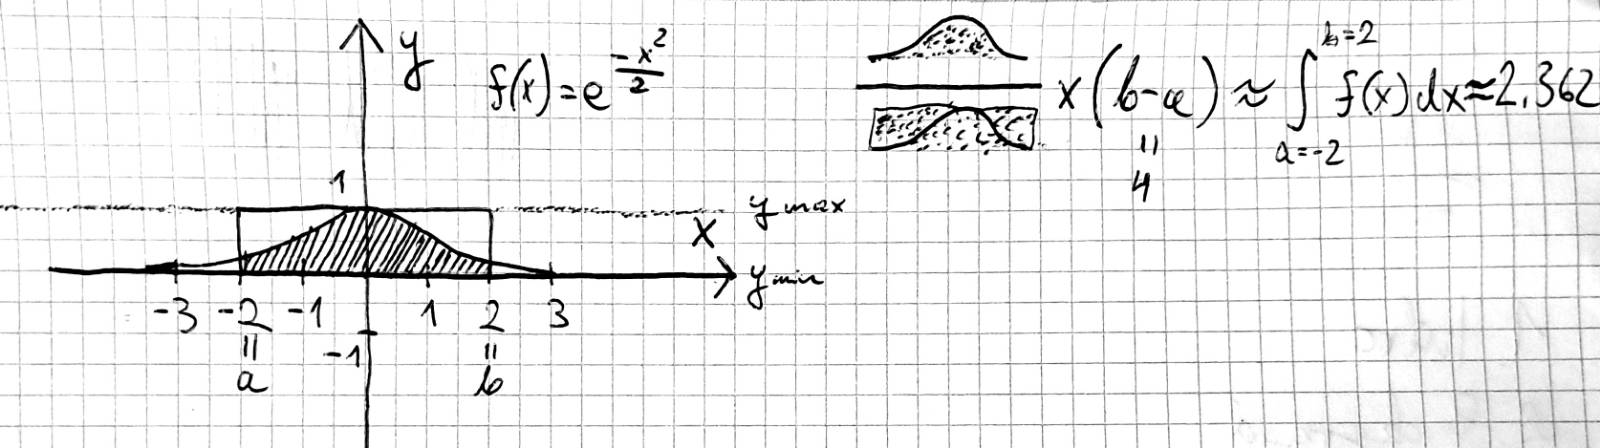
\includegraphics[width=12cm]{images/monte-carlo-integration-2.png}
    \caption{Monte Carlo integration example for $f(x)=e^{\frac{-x^2}{2}}$.}
    \label{fig:mc-integ}
\end{figure}

% The computation of Monte Carlo-based methods is very frequently accelerated with GPUs due to the high data independence of each sample, which have earned them the reputation of being "massively parallelizable". However, they have not been historically used in ray-tracing until relatively recently, as overviewed by Novák et al.~\cite{MonteCarlo} in 2018. The way Monte Carlo is typically applied in ray-tracing is when we're computing the ray bounced off of the hemisphere centered at an object's surface normal. In the classical approach, the bounced rays are all uniformly probable, which may introduce problems for GPU schedulers such as warp divergence. Furthermore, this might also involve many disk accesses of different models, leading to a noticeable overhead. Both of these problems have been addressed with the advancements in recent hardware such as the advent of ray-triangle intersection components in done by so-called RT (ray-tracing) cores and new algorithms for grouping the device threads into groups operating on similar areas of the scene.

The computation of Monte Carlo-based methods is frequently accelerated using GPUs due to the high data independence of each sample, which earned them the reputation of being "massively parallelizable." However, their application in ray tracing has been relatively recent, as discussed by Novák et al.~\cite{MonteCarlo} in 2018. 

In ray tracing, Monte Carlo methods are typically employed to compute rays that are bounced off a hemisphere centered around an object's surface normal. In classical implementations, these bounced rays are often sampled uniformly, which can lead to issues for GPU schedulers, such as warp divergence. Additionally, this uniform sampling may result in numerous disk accesses to different models, introducing significant overhead. Recent advancements in hardware, including dedicated ray-triangle intersection components found in ray tracing (RT) cores, along with new algorithms for grouping device threads that operate on similar areas of the scene, have addressed these challenges. These improvements enhance the efficiency of Monte Carlo methods in ray tracing, allowing for more effective utilization of GPU resources.

\subsection{Gaussian Mixture Modelling (GMM)}

Gaussian Mixture Modelling (GMM) is a technique used to approximate a probability density function (PDF) $ f: X \rightarrow [0,1] $ s.t. $X=\{x_1,\ldots,x_N\}$ as a weighted sum of $K$ Gaussian distributions (or Gaussians for short), where $K$ is determined automatically:

$$f(x) \approx \sum_{k=1}^{K} w_k \cdot g_k(x),$$

where for $d$-dimensional data, each Gaussian $ g_i(x) $ would be defined as:

$$g_k(x) = \mathcal{N}(x | \mu_k, \Sigma_k) = \frac{1}{(2\pi)^{\frac{d}{2}} |\Sigma_k|^{\frac{1}{2}}} e^{\left(-\frac{1}{2} (x - \mu_k)^T \Sigma_k^{-1} (x - \mu_k)\right)}$$

This idea generalizes to other kernels as well, bearing the name kernel mixture modelling. The weights $ w_k $, as well as the parametrization of the Gaussians, are determined via the Expectation-Maximization (EM) algorithm, which relies on two phases, as hinted by its name. The expectation phase computes the expected values of the latent variables, while the maximization phase updates the parameters to maximize the likelihood of the data in the Gaussian representation.

For a fixed point $x_n$ and Gaussian cluster $C_k$, we can define the probability of its observation within that cluster:

$$\mathbb{P}(x_n|w_k,\mu_k,\Sigma_k) = w_k \mathcal{N}(x_n | \mu_k, \Sigma_k) $$

The goal of the GMM algorithm is then to maximize the following function, which implicitly assumes that the distributions of points are pairwise-independent:

$$
\mathbb{P}(X | w, \mu, \Sigma) = \prod_{n=1}^{N} \left[ \sum_{k=1}^{K} w_k \mathcal{N}(x_n | \mu_k, \Sigma_k) \right]
$$

Given a new observation $x_n$, the posterior probability of belonging to the $k$-th component of the GMM is given as follows:

$$\gamma_{n,k} = \frac{w_k\cdot\mathcal{N}(x_n | \mu_k, \Sigma_k)}{\sum_{j=1}^{K} w_j\cdot\mathcal{N}(x_n | \mu_j, \Sigma_j)},$$

It's easy to see that the count of points pertaining to the $ k $-th component is:

$$N_k = \sum_{n=1}^{N} \gamma_{n,k}$$

Maximizing $ \mathbb{P}(X | \pi, \mu, \Sigma) $ with respect to its parameters gives:

$$\mu_k = \frac{1}{N_k} \sum_{n=1}^{N} \gamma_{n,k} x_n$$

$$\Sigma_k = \frac{1}{N_k} \sum_{n=1}^{N} \gamma_{n,k} ||x_n - \mu_k||^2$$

$$w_k = \frac{N_k}{N}$$

Thus, we can see that $ \mu_k, \Sigma_k, $ and $ w_k $ depend on $ \gamma_{n,k} $, and conversely, $ \gamma_{n,k} $ also depends on $ \mu_k, \Sigma_k, $ and $ w_k $, resulting in a circular dependency. To resolve this, we iteratively optimize both sides as follows:

\begin{enumerate}
    \item Initialize $ \mu_k, \Sigma_k, w_k $.
    \item Compute $ \gamma(z_{n,k}) $ for all $ n, k $.
    \item Recompute $ \mu_k, \Sigma_k, w_k $, and return to step 2.
\end{enumerate}

The final approximation of $f$ that we obtain as a GMM allows us to easily compute various properties of the distribution, including the integral of $ f $ over a given region with a closed-form equation:

$$\int_{A} f(x)~dx\approx \int_{A}\left(\sum_{k=1}^{K} w_k \cdot g_k(x)\right)~dx = \sum_{k=1}^{K}\left(w_k\cdot \int_A g_k(x)~dx\right)$$,

where $A$ is the region of interest. In particular, if $ A $ is the entire space, then $\forall_{k=1\ldots,K}~\int_Ag_k(x)~dx=1 $, leading to:

$$
\int_{\mathbb{R}^d} f(x) \, dx = \sum_{k=1}^{K} w_k = \frac{N}{N} = 1,
$$

which confirms that the GMM is a valid probability density function.

\subsection{Structure from Motion (SfM)}
TODO

\section{Graphical techniques}

\subsection{Ray-Tracing (RT)}

Ray-tracing is a rendering framework whose basis is the simulation of light travel by modeling it as a sequence of interactions of light rays with the surface of objects, such as absorption and reflection, much like what happens in real life. Contrary to real life however, the rays travel not from the light source to the eye, but from the eye to the light source. This seemingly insignificant change makes all the difference for an efficient implementation of the phenomenon, as it saves up computations on rays that contribute nothing to the visible part of the scene being observed.

A ray $\bm{r}$ can be mathematically defined by the following equation:
$$\bm{r}(t) = \bm{o} + t\bm{d},$$
where $\bm{o}$ is the ray's origin, $d$ the direction of the ray and $t$ parametrizes the distance traveled. A classic example of how this is used is checking whether a ray intersects a sphere centered in $\bm{c} = (c_x,c_y,c_z)$ with radius $r$. It is easy to see this boils down to solving for $t$ in the following equation:
$$||\bm{c} - \bm{r}(t)||^2 = r^2$$

The equation that is most characteristic of ray-tracing however is the famous "rendering equation":
$$L_o(\bm{x}, \bm{\omega_o}, \lambda, t) = L_e(\bm{x}, \bm{\omega_o}, \lambda, t) + \int_{\Omega}f_r(\bm{x}, \bm{\omega_i}, \bm{\omega_o}, \lambda, t) \cdot L_i(\bm{x}, \bm{\omega_o}, \lambda, t)\cdot||\bm{\omega_i}, \bm{n}||^2~d\bm{\omega_i}$$

Above, $L_o$ is the total outgoing light, $L_e$ is the emitted light, $f_r$ is the bidirectional reflectance distribution function (BRDF) and $L_i$ is the light reflected by the surface.  The BRDF, $ f_r(\omega_i, \omega_o) $, describes how much light incoming from direction $ \omega_i $ is reflected in the direction $ \omega_o $ at a given point on the surface. $\Omega$ is the hemisphere of the surface on which the ray lands, centered at the surface normal $\bm{n}$ (the unit vector perpendicular to it) and the integral on it corresponds to taking into account all the possible outgoing rays. In practice, this integral is never computed directly, but rather estimated in a Monte Carlo manner by sampling a few rays and performing a discrete mean over them. This numeric approximation can be further optimized by importance sampling, which involves tracing more rays in the immediate direction of a light source rather than dimmer areas.

The rendering equation encapsulates the fact rays bounce off of surfaces and thus trace a path, illuminating many objects. When implementing ray-tracing we do not allow for an indefinite number of bounces, but limit them to a certain threshold and also account for the degree of absorption of light by different surfaces, which can result in a total absorption of the ray after a couple bounces.

Ray tracing has several variations, one of which is path tracing, a technique that produces higher-fidelity images by modeling global illumination. Unlike standard ray tracing, which focuses on direct light interactions, path tracing follows rays as they reflect and refract multiple times throughout the scene. This method accurately represents complex light behaviors, such as color bleeding and soft shadows, by generating multiple secondary rays upon surface interaction. Although path tracing requires more computational resources and samples to achieve noise-free images, it delivers more photorealistic results, making it a popular choice for high-quality rendering in film production and architectural visualization.

\subsection{Rasterization}
Rasterization is one of the earliest developed and most efficient rendering methods, widely utilized in real-time applications, particularly in video games and interactive simulations due to its ability to leverage the parallel processing capabilities of modern graphics hardware (GPUs). In fact, this method is so predominant that most graphics engines up to 2015 were based on rasterization. This process converts 3D images defined by triangular meshes into a raster image (a grid of pixels) by projecting them onto a 2D plane for display on screens.

The technique begins with vertex processing, where the 3D coordinates of the vertices are transformed into 2D screen space using projection matrices. This step also includes operations such as lighting calculations and texture coordinate generation. Once the vertices are processed, the next phase involves triangle setup, where the bounding box of each triangle in screen space is determined, and edge equations are calculated to prepare for rasterization.

During fragment generation, the algorithm checks each pixel within the bounding box to see if it lies inside the triangle using interpolation methods. If a pixel is inside, a fragment is generated that contains interpolated attributes, including color, texture coordinates, and normals. A critical component of this process is the depth buffer algorithm, which manages the visibility of objects by tracking the depth of each pixel on the screen, indicating the distance from the camera. When a triangle is rasterized, the algorithm compares the depth of the triangle's fragments against the current values stored in the depth buffer. If a fragment is closer to the camera than the existing pixel value, the pixel's color and depth are updated; otherwise, the fragment is discarded. This mechanism ensures that only visible surfaces are rendered, effectively handling occlusion within the scene.

After all triangles have been rasterized, additional post-processing techniques such as anti-aliasing, tone mapping, and various filters can be applied to enhance the final image, culminating in an approximation of the scene's illumination.

While rasterization does not inherently simulate the complex interactions of light as ray tracing does, it can still produce visually appealing results, especially when combined with techniques like texture mapping, shading, and shadow mapping. These methods help approximate realistic lighting effects while maintaining reasonable rendering times. Overall, rasterization remains a fundamental technique in the field of computer graphics, enabling real-time rendering of complex scenes.

\subsection{Spatial Acceleration Structures}

Given the complex nature of the physical behaviors that ray tracing aims to emulate, optimizing this process is crucial for enhancing both render time and quality. Classical, unoptimized ray tracing involves iterating over all triangles in a scene represented by 3D triangle mesh models and calculating ray-triangle intersections for each triangle. This approach is highly inefficient, particularly in complex scenes with numerous models or highly detailed geometries.

To address this inefficiency, spatial acceleration structures are employed. These auxiliary data structures are designed to reduce the number of triangles that need to be checked for intersection. The simplest form of such a structure is a regular cubic grid, which uniformly partitions the model. However, this method is not ideal, as it does not account for the distribution and clustering of data points, leading to poor space utilization and slow query times. 

Quadtrees and octrees improve upon this basic approach by avoiding the storage of empty grid cells, effectively pruning child nodes that do not contain any triangles during the tree construction process. 

Despite this improvement, some nodes may still be densely populated while others remain sparsely populated. This is where Binary Space Partitioning (BSP) trees come into play. BSP trees recursively split the object using hyperplanes based on specific policies, such as spatial or object median, ensuring a more even distribution among the cells. K-d trees are a specialized form of BSP trees where each hyperplane is axis-aligned (perpendicular to one of the coordinate axes), which can simplify computations.

\subsubsection{Bounding Volume Hierarchy (BVH)}

\begin{figure}[htp]
\centering
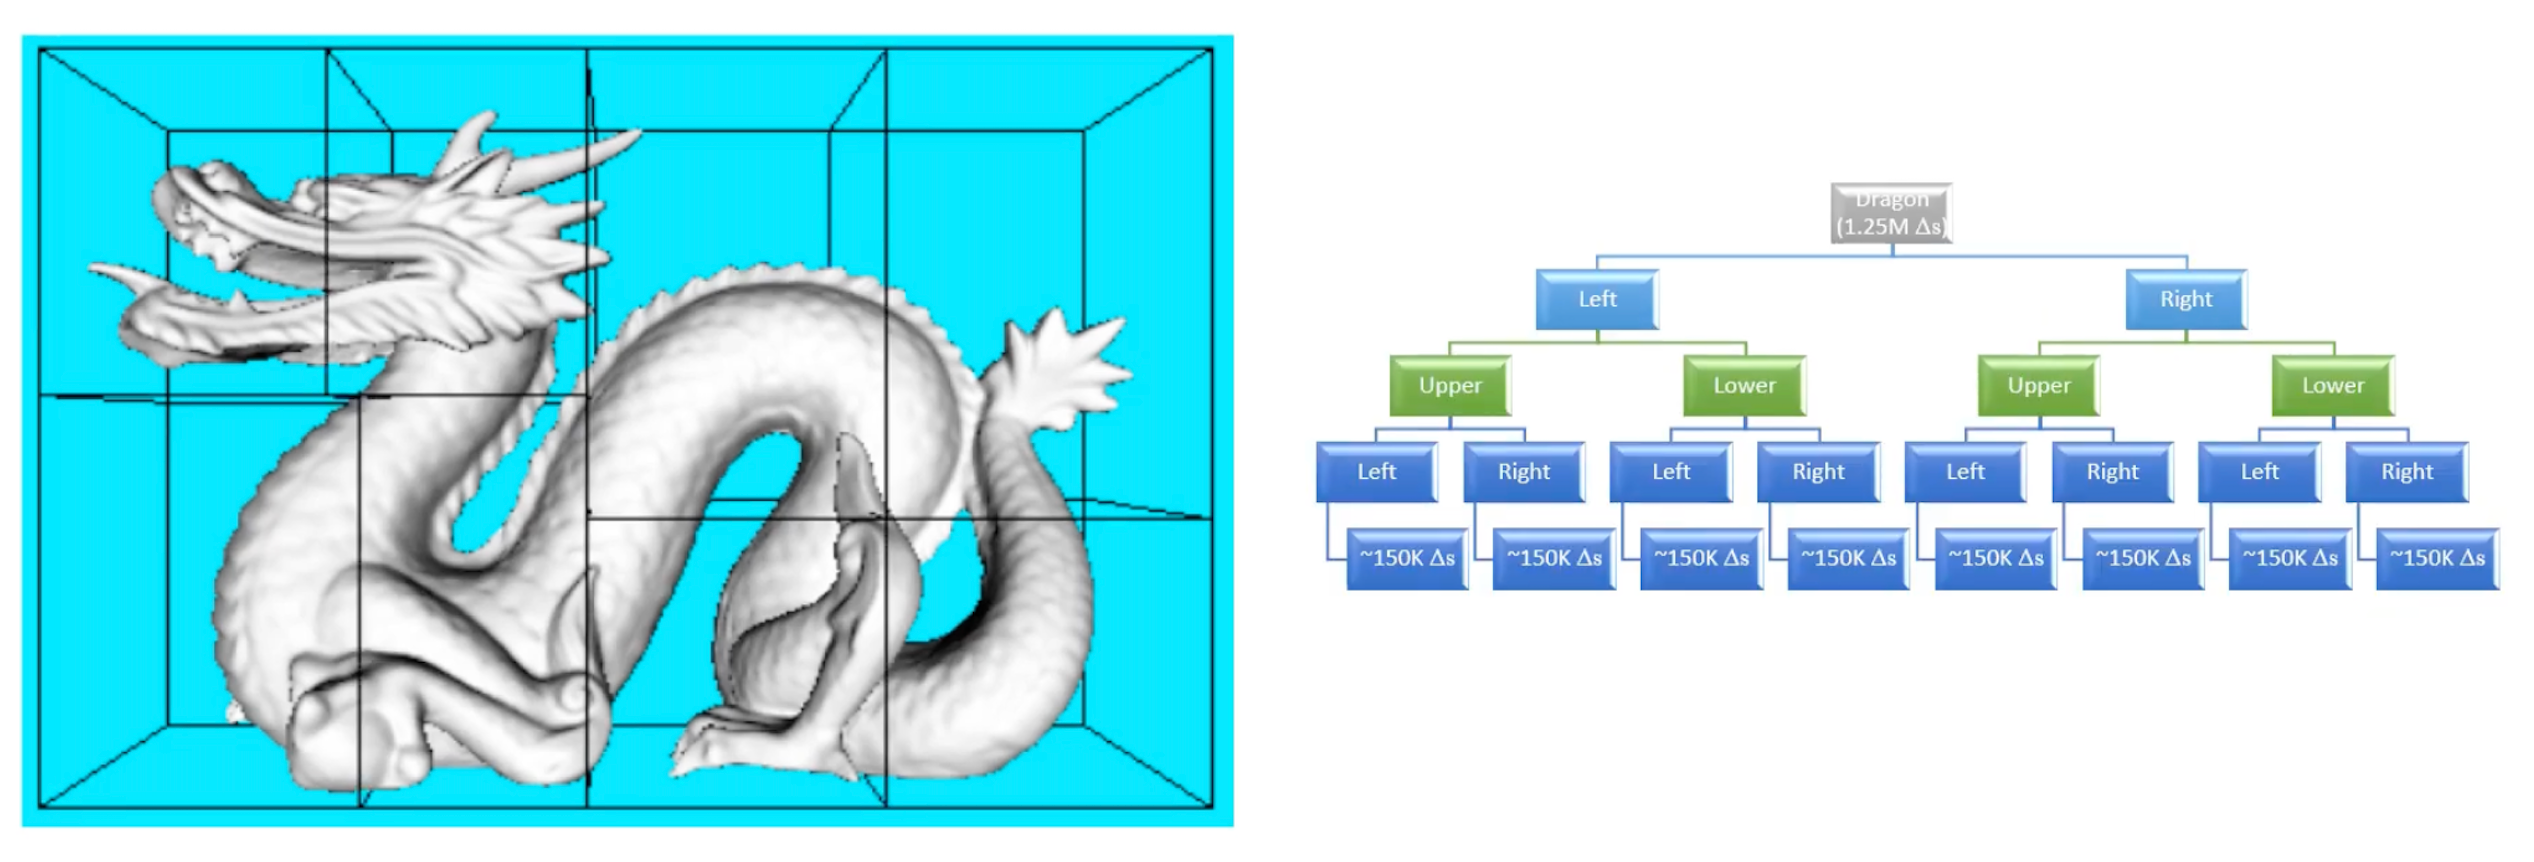
\includegraphics[width=12cm]{images/bvh-dragon.png}
\caption{A BVH of depth 5 applied to the Chinese Dragon model~\cite{ChineseDragon}.}
\label{fig:bvh-dragon}
\end{figure}

Ultimately, the Bounding Volume Hierarchy (BVH~\cite{SpatialAccelerationStructures}) has emerged as the most commonly used structure for our purposes, introducing the concept of bounding volumes. The fundamental idea behind them is to encapsulate objects in the scene with simpler geometric shapes, typically boxes or spheres, that are easier to test for intersection than the actual objects being rendered. By constructing these bounding volumes, we can quickly determine if a ray intersects them; if a ray does not intersect a bounding volume, it cannot intersect any of the objects contained within it.

In the ray tracing process for BVHs, we first check for intersection with the bounding volume. If there is no intersection, we can disregard all objects within that volume. Conversely, if an intersection occurs, we then check at which half of the bounding volume did it happen and recurse for it. The heuristic for splitting the volume into the two halves is often a median in terms of the number of points or their coordinates. This recursive process continues until a specified depth is reached, at which point standard ray-triangle intersection tests are performed, but on a significantly smaller subset of triangles. Determining the optimal depth and establishing an upper limit for the number of triangles within a leaf node is typically done through experimentation and might depend on the model. 

In summary, the BVH is an efficient data structure that is easy to understand, inexpensive to compute and store, and significantly accelerates the ray-triangle intersection process, making it a vital tool in the realm of ray tracing. It is widely used as a foundation to other solutions, such as OpenVDB~\cite{OpenVDB}. It was also used in the implementation of the "3D Gaussian Splatting for Real-Time Radiance Field Rendering"~\cite{3DGS} paper.

\section{Gaussian Splatting (GSplatting)}

Gaussian Splatting (GSplatting), whose original paper was published in just 2023, represents a novel approach in the realm of 3D scene reconstruction, going beyond the already impressive advancements made by NeRFs. How GSplatting primarily distinguishes from its predecessor is that it provides an explicit rather than black-box representation of the generated scene, saving up on computations and allowing for direct manipulation.

\begin{figure}[htp]
    \centering
    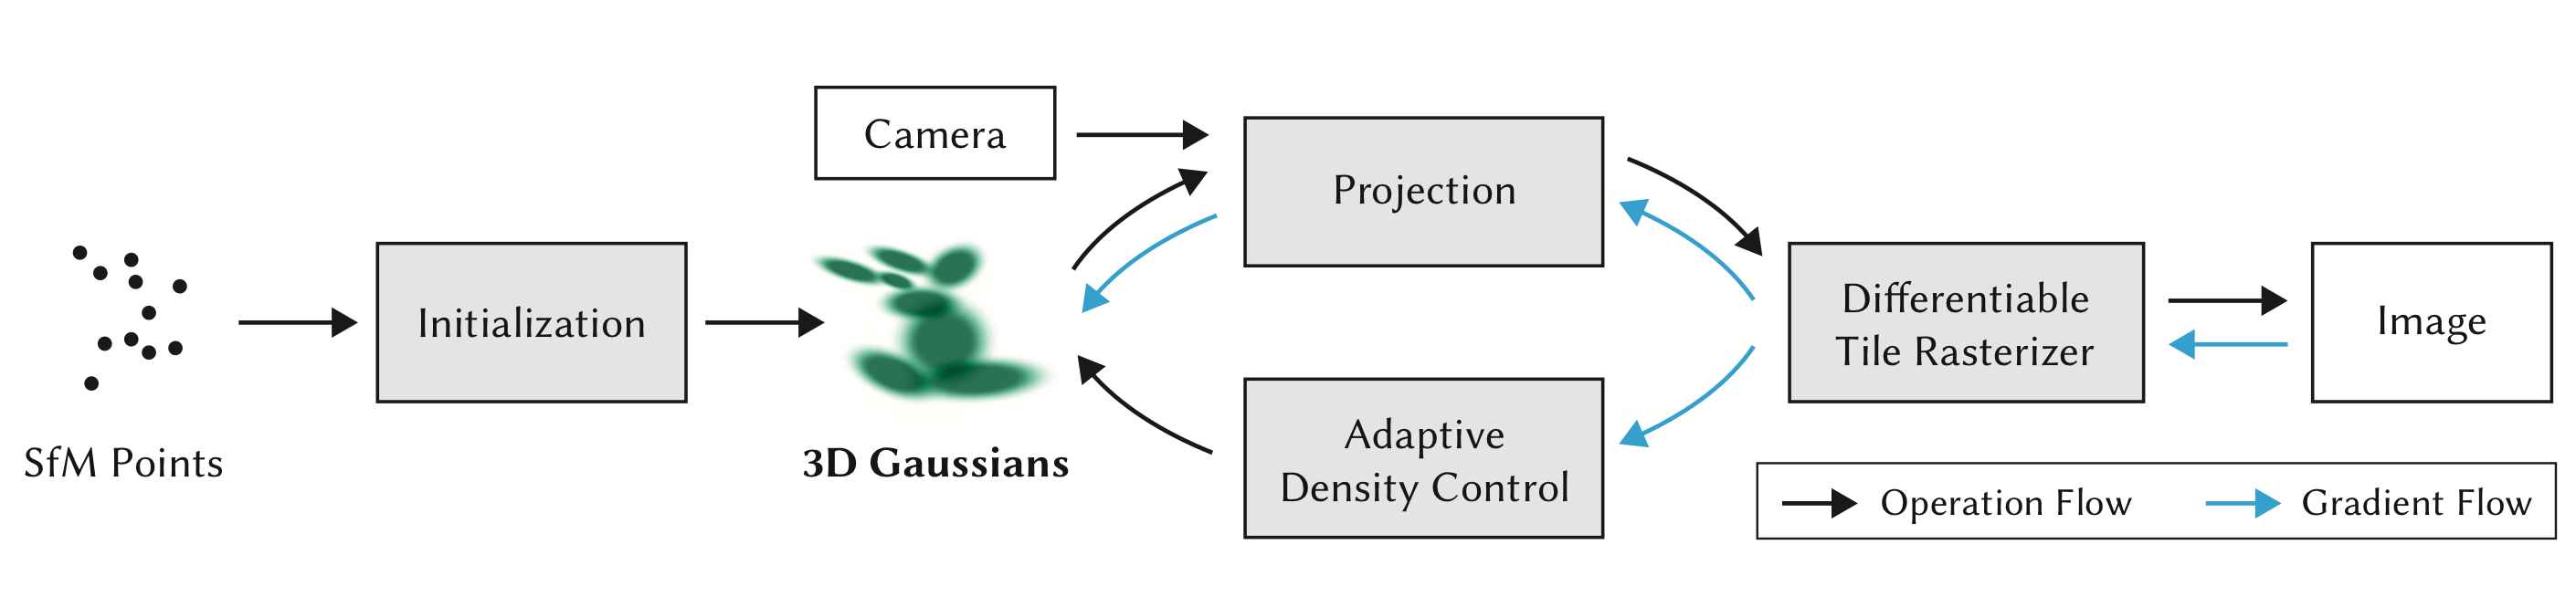
\includegraphics[width=12cm]{images/gsplats-pipeline.png}
    \caption{Rendering and optimization pipelines of Gaussian Splatting.}
    \label{fig:gsplats-pipeline}
\end{figure}

The GSplatting pipeline, as portrayed in figure~\ref{fig:gsplats-pipeline} begins with capturing a series of photographs from various angles, similar to traditional photogrammetry methods. Subsequently, a mathematical technique known as Structure from Motion (SfM) is employed to estimate a sparse 3D point cloud from the differences observed in these images. Each point in the 3D point cloud is then mapped to a Gaussian, which can be visualized as a bell-shaped curve in 2D and an ellipsoid in 3D. Since these primitives are differentiable, they are suitable for a gradient descent-based optimization strategy of their parameters including position, size, color (given by so-called spherical harmonics), orientation and opacity to minimize the difference between the output they render and the original 2D images. 

Furthermore, a technique called adaptive density control is incorporated into the training process to enable fine-grained capturing of details (e.g. leaves of a tree) while conserving computations for less relevant sections of the model (e.g. the sky). It revolves around ridding the model of splats that are too transparent, splitting ones that are too big into smaller ones, or performing the inverse operation to form a bigger Gaussian.

Traditionally, the rendering pipeline in GSplatting employs rasterization techniques. According to the viewer's perspective, all Gaussians are first sorted by depth in the field of view, which is often the most computationally intensive part of the process. Then, they are projected onto the 2D viewport and alpha-blended together.

This technique has demonstrated impressive performance, achieving high fidelity even at frame rates of up to 144 FPS for complex scenes, outclassing NeRFs by many orders of magnitude. This efficiency is particularly beneficial for applications in real-time environments, such as virtual and augmented reality, where rapid rendering is crucial. Furthermore, GSplatting has been integrated into various platforms, including Unity and Unreal Engine, as well as AR applications for iOS and Metal, and WebGL viewers.

Despite its advantages, GSplatting faces challenges, particularly in handling complex lighting scenarios and transparency effects. The baked-in color of each splat limits the ability to change lighting dynamically unless advanced techniques like ray tracing with a Bounding Volume Hierarchy (BVH) are employed. Approaches like this have been proposed and explored by Condor et al ~\cite{DSYG}.

In summary, Gaussian Splatting represents a significant advancement in the field of 3D graphics, offering a robust framework for creating detailed and editable 3D scenes from 2D images. Its applications span various domains, including augmented reality, architectural visualization, medical imaging, and digital preservation of cultural heritage sites, making it a versatile and impactful technique in contemporary computer graphics.

\section{Gaussian Mixture Modelling for Volumetric Ray-Tracing}

During the optimization loop of the GSplatting pipeline~\ref{fig:gsplats-pipeline}, a process called EWA splatting is done for each input view of the scene before the rasterization stage, which involves projecting the corresponding view of the 3D Gaussian mesh into 2D, implying the 2D projection of the bounding ellipsoid (or shell) of each Gaussian primitive. Unfortunately, if the Gaussian is anisotropic and hence represented by a non-diagonal covariance matrix, then the projection is no longer Gaussian. Should that happen, we create a new Gaussian to approximate this projection with a mean centered inside of it and the covariance defined by the principal axis. Since the original Gaussian's projection changes depending on the view, and the optimization of each view is equally accounted for in the gradient update, this leads to inconsistencies when inspecting the scene through a trajectory. Namely, some Gaussians may flicker or pop out of their mesh when changing perspectives~\ref{fig:flicker}, giving away the underlying representation and being detrimental to a realistic experience of the scene.

\begin{figure}[htp]
    \centering
    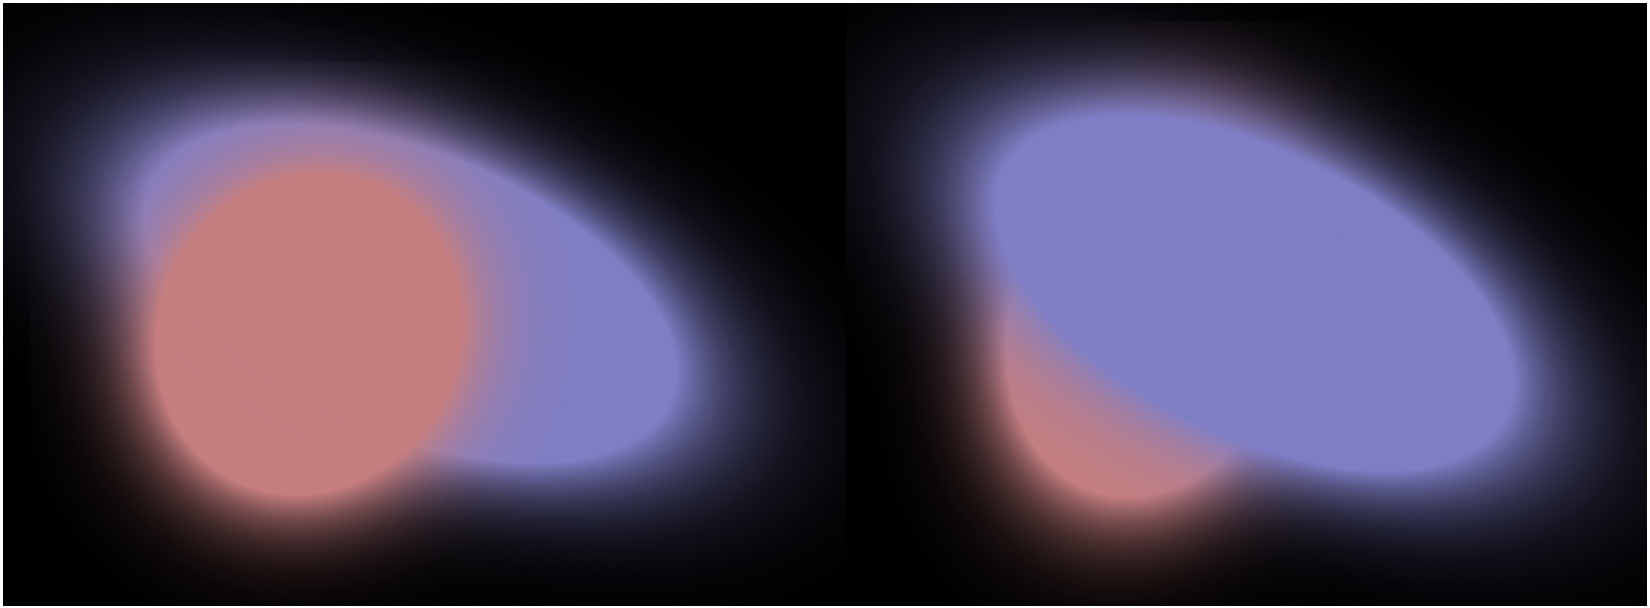
\includegraphics[width=12cm]{images/flicker.png}
    \caption{Flickering artifacts of Gaussian kernels in the standard approach.}
    \label{fig:flicker}
\end{figure}

Condor et al.~\cite{DSYG}, as early as in their paper's title, suggest that this might not be needed and explore an alternative option. They suggest that the approximation of the density function, followed by the rasterization stage is not needed, and that the usage of a closed-form solution to the volume density can be used, enabling the use of ray-tracing as the rendering method. Indeed, they show that Gaussian Mixture Modelling can be used to obtain said solution, as illustrated in figure~\ref{fig:gmms}.

Ray-tracing the Gaussian mesh offers significant advantages in rendering, primarily through its ability to accurately model complex light behaviors such as reflections, refractions, transparency, translucency, and shadows. This results in a more realistic representation of scenes, capturing nuanced lighting effects like caustics and global illumination that traditional rasterization methods often struggle to achieve, especially for volume rendering. Additionally, ray tracing enables dynamic, real-time changes in illumination, enhancing interactivity in applications like video games and virtual reality, where lighting conditions can shift based on user interactions.

\begin{figure}[htp]
    \centering
    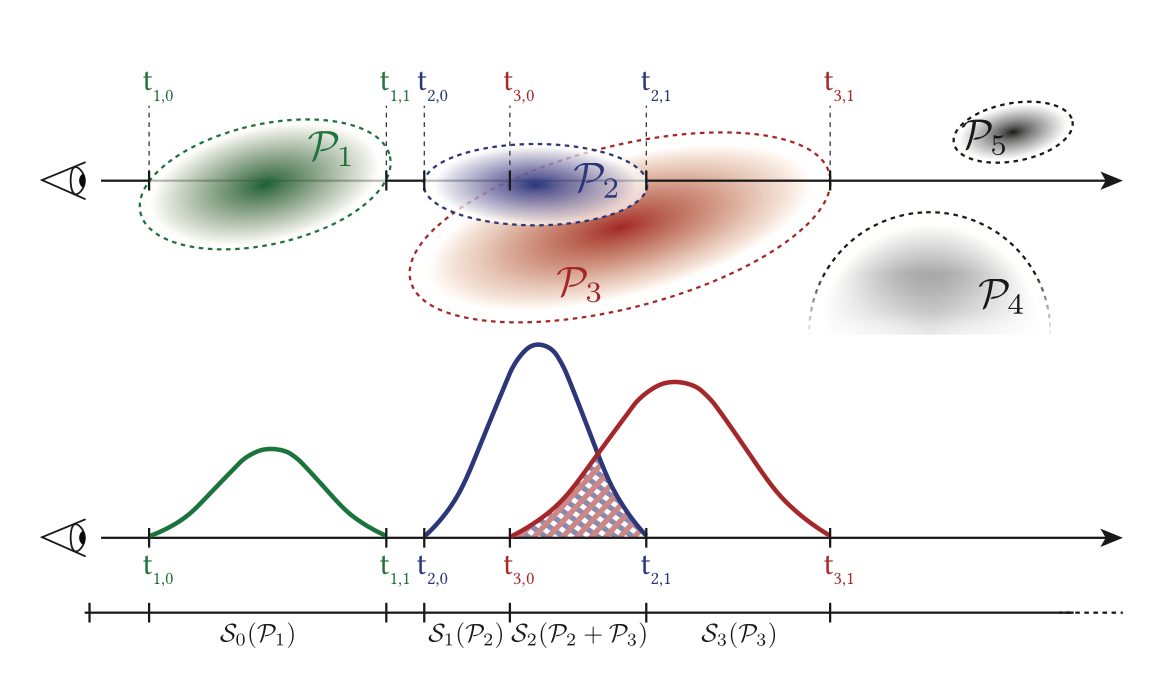
\includegraphics[width=12cm]{images/dsyg-gmms.png}
    \caption{Usage of GMMs in in a ray-traced scene view. Conveniently, the area on which $\mathcal{P}_2$ and $\mathcal{P}_3$ overlap can be analytically computed.}
    \label{fig:gmms}
\end{figure}

Furthermore, Condor et al. explore Epanechnikov kernels~\ref{fig:kernels} as an alternative to Gaussians:

$$\mathcal{E}(\bm{x})=\begin{cases}
    \frac{15}{56\pi\sqrt{(7|\Sigma|)}}(1-\frac{1}{7}(d(\bm{x}))&\text{if } d(\bm{x})\leq 1 \\
    1 &\text{otherwise,}
\end{cases}$$

\begin{figure}[htp]
    \centering
    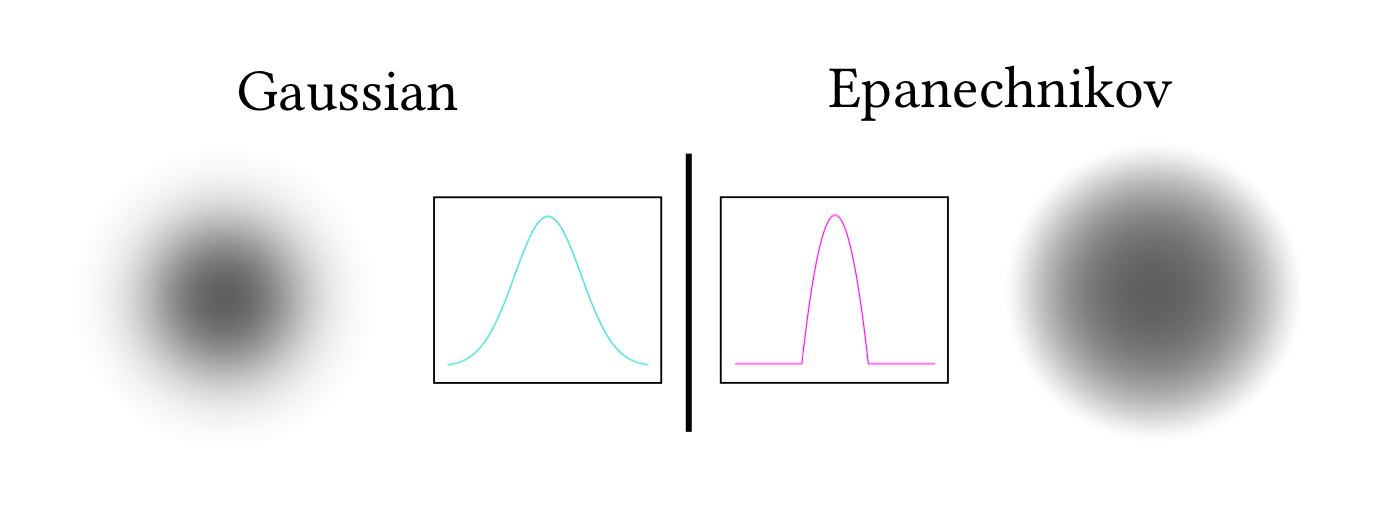
\includegraphics[width=12cm]{images/dsyg-kernels.png}
    \caption{Visual comparison between 1D Gaussian and Epanechnikov kernels.}
    \label{fig:kernels}
\end{figure}

where analogously to Gaussians, $\Sigma$ is a $3\times3$ covariance matrix, $d(x)=(\bm{x}-\bm{\mu})^T\Sigma^{-1}(\bm{x}-\bm{\mu})$ and $\mu$ is the mean. Using these kernels to model a scene typically involves using them in larger amounts than Gaussians, the resulting Epanechnikov primitives being smaller. This can lead to a better utilization of the underlying BVH structures of the 3D models they fit, which perform better for a more fine-grained layout of primitives. These kernels also differ from Gaussians in how they sharply decay to $0$, which on average leads to less overlaps in the mesh they form. This has two consequences. Firstly, the resulting scene can be modelled more accurately, especially if it's highly detailed. Secondly, the number of primitives along the path of a ray is on average reduced, which speeds up computations. Indeed, Condor et al. showed that Epanechnikov kernels often outperform Gaussian kernels in terms of both rendering speed and visual quality.

Overall, the performance of this new approach is comparable to the original by Kerbl et al.~\cite{3DGS} in terms of quality, while allowing to reap all the benefits from ray-tracing, including the in-real-time relighting of the scene. The speed in terms of FPS is almost 40\% of the original, which is still faster than any NERF-based approach, however this can be further improved, for instance by improving the underlying renderer.

\section{Planned contributions}

\subsubsection{Scope}

The goals of the thesis is twofold. First, it is to implement an open source, highly optimized path tracer in CUDA/C++ for kernel mixture volumes that allows for real-time rendering. Secondly, it is to use it to perform further extensions of the work of Condor et al. within the "Don't Splat Your Gaussians"~\cite{DSYG} paper. 

Possible extensions include:
\begin{itemize}
    \item experimenting with different representations of the the Gaussians for ray-tracing compared to the currently used BVH,
    \item a generalized way to handle emissive and absorptive kernels for a unified model that takes advantage of closed form integrals for accurate product sampling of light sources and BSDFs,
    \item SGGX and novel microflakes models to support efficiently surface-like materials in a unified way,
    \item parametric kernels that enable more efficient, compact and accurate radiance fields,
    \item Lagrangian methods for fluid dynamics simulations to directly transform them into kernel mixture models for rendering, without the need of discretization into voxel grids and running kernel regression.
\end{itemize}

\subsubsection{Approximate Timeline}

The approximate 7-month timeline that we devised with my supervisors, effective from the date I formally agreed to undertake the project (07.11.2024) is as follows:

\begin{itemize}
  \item[\checked] \textbf{weeks 0-3:} literature review on rendering, path tracing, rasterization and related papers to DSYG~\cite{DSYG} and 3DGS~\cite{3DGS},
  \item[\unchecked] \textbf{weeks 3-12:} implementation of DSYG, ideally, with SLANG.D~\cite{SLANG.D} \& Optix~\cite{Optix} shaders that compile into CUDA kernels, so that we can run inverse rendering tasks without analytic derivatives, or directly in CUDA with analytic backward passes,
  \item[\unchecked] \textbf{weeks 12-24:} exploration of one of the potential extensions,
  \item[\unchecked] \textbf{weeks 24-28:} thesis writeup and review.
\end{itemize}

The project is currently in its second stage in which I am writing a path tracer based on resources available online~\cite{RTI1W}.

If the exploratory stage is fruitful, we envision it being submitted as a publication in a top graphics/vision conference such as HPG, EGSR, SIGGRAPH, EUROGRAPHICS, CVPR or ICCV/ECCV.

%%%%%%%%%%%%

% Graphics engines  up to 2015 were mostly based od rastrizing. They had little control over ow you can mode light transport and they were mostly based on CPUs except of the Arnold renderer

% Delta-tracking

% Ray-marching
% Ray-marching, as opposed to ray tracing that precisely calculates intersection points by using distance functions to gradually step into the scene until an object is hit

% VDB
% \section{VDB}

% - Voxel [ = Volume + Pixel ]
%     - Smallest addressable unit of index space
%     - Resides at the leaf node level
% - Tile
%     - Larger constant domain
% of index space
%     - Resides at the upper (non leaf) tree levels
% - Active state
%     - All values (voxels and tiles) have a binary state
%     - Interpretation of state is application-defined

% Ray-tracing, most often, visits neighbors and this high spatial locality of the structure is perfect for that


% delta-tracking (used in physical simulation, newton transport physics, triple A studios, movie studios) is unbiased, ray-marching and denoisers      is biased. There is a trade off low-variance and fast convergence => some bias (example - denoisers). High variance means low confidence, no rush, run many samples, you'll get your integral value. 

% The past 20 years in graphics people were doing voxel grids they were doing research on continuous volume, delta tracking, optimizing delta tracking. The Novak paper illustrates how 

% TODO:
% Spherical harmonics (optional) to represent all view-dependent effects and lighting - changing color when viewing from a different angle, also glint and vineer, specularities. You only optimise the base color at first and slowly add higher frequency bands over time 

% Ideas:
% - 3d memory capture, spatial media
% - reality bending art: 2290
% - relightability
% - capturing UNESCO landmarks
% - AI compatible with meshes is being researched 
% - augmented reality
% - architecture
% - medical imaging: 3d renderings of organs from 2d scans
% - construction sites


% $L(x, \omega) = L_e(x, \omega) + \int_{S^2}L(x, -\omega')f(\omega,\omega')|n\cdot\omega'|d\omega'$

% \section{Synthetic Scenes}

% \section{SRNs}
% Scene Representation Networks implicitly represent a scene using a FC NN. They have issues with multi-view consistency and can't represent high-frequency details

% \section{LLFF}
% Local Light Field Fusion uses a pretrained network to promote each input view to a high-res 3d volume. LLFF blends multiple renderings with limited FOVs, resulting flickering artifacts due to inconsistencies along image borders, between adjacent volumes

% \section{NV}
% Neural Volumes encode a scene as a 128-cubed voxel grid and use a warp-field to better allocate these limited samples. They still are unable to represent fine-detail

% \section{Real Scenes}
% SRN uses a RNN to rainmarch through encoded scenes resulting in inconsistent 


% Other innovations:
% - they used this to make videos with an NN (TODO: source)
% - 3D scanning. KIRI - gaussian to 3d mesh for 3d modelling (scan and remove background to isolate model), addons for Blender
% ply file.
% - deformation fields to make video with a small, fast NN since many points move together


% YouTube:
% https://youtu.be/BmbfjHoqKUs
% https://youtu.be/MzUxOe5x24w
% https://youtu.be/Sxy7tcRZh-8
% https://youtu.be/C708Mh7EHZM
% https://youtu.be/jV1g5OY0L5s
% https://youtu.be/917WVr2EHh4
% https://youtu.be/IUEzsWOOErE
% https://youtu.be/CRlN-cYFxTk
% https://youtu.be/JuH79E8rdKc
% https://youtu.be/CRlN-cYFxTk
% https://youtu.be/s3PHOPv88P4
% https://youtu.be/KFOy354zf9E
% https://youtu.be/5SQ9pJS3S5I


% Ideas/keywords
% - backface culling

% Stack Overflow
% - https://computergraphics.stackexchange.com/questions/14132/when-to-apply-backface-culling-depending-on-the-ray-and-material-type
% - https://stackoverflow.com/questions/66847292/bidirectional-path-tracing-algorithm-explanation
% - https://computergraphics.stackexchange.com/questions/7828/difference-between-bvh-and-octree-k-d-trees
% - https://computergraphics.stackexchange.com/questions/14132/when-to-apply-backface-culling-depending-on-the-ray-and-material-type
% - https://www.reddit.com/r/GraphicsProgramming/comments/yha34i/difference_between_vdb_and_bvh/    

% Ray marching - like ray-tracing with a step
% Woodcock tracking/delta tracking

% $result = exp(distancee * ABSORPTION)$


% • Volume
% - y =f(x) where x is (x, y, z)
% - Standard VDB: value y is stored (discretized/sampled) at voxels


% https://youtu.be/y4KdxaMC69w